\subsection{Field Cage for protoDUNE Dual Phase}~\label{sec:proto-dune-dp-fc}
Field cages provide uniform electric fields for ionization electrons to drift to anodes for the detection in the Time Projection Chamber.
The baseline design for DUNE LArTPC is that of the single phase in which the ionization electrons created by the secondary particles 
resulting in neutrino-nucleon interactions drift in LAr and get detected on the anode plane that resides inside the liquid phase of argon.  An alternative technology is the LArTPC that the ionization electrons drift through LAr but then extracted through the strong extraction field at the top of the liquid and detected in the anode in gaseous phase of argon after a signal amplification via an large area gas electron multiplier (LEM), hence the dual phase.  While the DUNE baseline design technology is single phase, the dual phase detector provide a complementary techology for the fact that it uses pixelated anode readout structure that eliminates the confusion in the hit coming from the ghost hits in wire based detector.

During the period of his sabbatical stay at CERN, Yu begun to work on WA105, a dual phase $6m\times 6m\times 6m$ prototype testing project at CERN through the participation in the smaller prototype cosmic ray detector in $1m\times 1m\times 3m$.  This work provided an opportunity for UTA I.F. group to join WA105 as the first U.S. group and to position itself well to play a leading role in dual phase detector technology.   Despite the fact that the dual phase technology is currently at a lower priority to the single phase LAr TPC, it is clear that U.S. groups' participation in this alternate and complementary technology is beneficial in many perspectives, including that of strengthening the international nature of DUNE collaboration an essential ingredient in its success.

As the schedule for DUNE experiment and for the two protoDUNE experiments get clearer, it became apparent that UTA will be able to play an importnat role in design and construction of these experiments.   The overarching strategy in identifying the construction project was to ensure UTA's contribution to any of the two protoDUNE experiments would enable direct participation in DUNE from the first 10kt module in early 2020's.  One such component easily identifiable is the field cage (FC) for which the collaboration is targeting to utilize as much common components as possible for SP and DP protoDUNE detectors.  With this premise, Yu has discussed with the DUNE management and has agreed to take the responsibility in design and construciton of DP FC together with the University of Zurich group, CERN and Fermilab.

Figure~\ref{fig:if-dp-fc} shows the current conceptual design of FC for the DP protoDUNE experiment.   The primay concept of this FC is to use a compartmentalized structure of submodules that consist of several straight profiles to provide voltage differentials for the generation of uniform fields. The use of straight profiles made of either aluminium or stainless steel makes the preassembly and shipment of submodules convenient. Each of these submodules will be prepared to the quality to hold high voltages at 180kV (for single phase) or  300kV (for dual phase) over the drift length.  
\begin{figure}[htb]
\centering
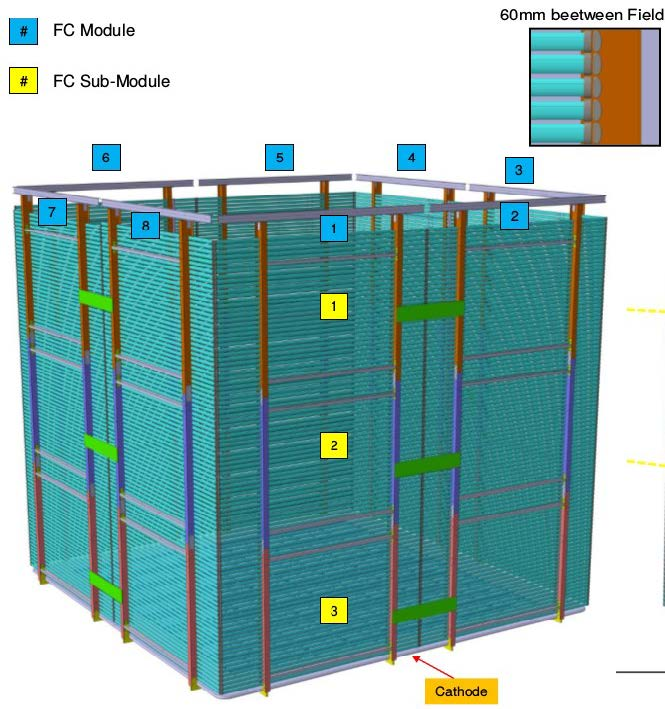
\includegraphics[width=0.50\textwidth]{images/if-dp-fc.jpg}
\caption[]{Conceptual schematic drawing of the field cage assembly for dual phase protoDUNE. Three submodules make up one module, two of which covers $6m\times 6m$ side. }
~\label{fig:if-dp-fc}
\end{figure}

At present, it has been agreed that either CERN or Fermilab will be responsible for purchasing and production of the necessary mechanical parts, including the I--beams that act as the spine of the submodule and the each profile.  The project funds will pay for the purchase electrical parts - voltage divider resisters and varistors for surge arresting - and the production of electronic boards the field cage.  UTA will work with the single phase field cage group, including BNL team, and the single phase field cage electronics group at Louisiana State University as well as the University of Zurich group on design of both the mechanical and electrical part of the dual phase field cage.   We will be responsible for pre-assembly of the field cage submodules, mounting of the electric boards, testing of each submodules and performing functional prototype testing with as large a field cage as possible before shipping the dissembled submodules out to CERN for installation.

For the completion of the design of the DP FC, our postdoctoral fellow, Animesh Chatterjee will be stationed at CERN starting from October 2016 through mid January 2017.   During this period, Chatterjee will work with the ETH and CERN groups to finalize both mechanical and electrical design of the FC for DP protoDUNE and ensure as much a commonality as possible with that of the SP.  Once these design parameters are agreed with the SP FC groups, a production could proceed.  The parts for the DP FC will be shipped to UTA for the quality control and preparation of each of the parts, assembly of submodules, mounting of electrical components, and electrical and mechanical testing for a submodule qualifications. A sizeable functional prototype FC of $6m\times 6m$, an electrically independent unit, will be put together and be subject under high voltage, though it may not be as high as 300kV given that the testing will be performed in air.  Once the functional testing completes, the functional prototype will be disassembled and the submodules will be shipped to CERN for the installation.

Since protoDUNE time scale has a hard limit of completing the beam data taking before the LHC heavy ion run in October 2018, it is essential for our group to operate under this time restriction in mind as presented in the strategic plan in section~\ref{sec:strategic-plan}.  To meet these goals, Yu plans on staying at CERN bottom half of 2017, utilizing the remaining funds from the agreements with LAPP and ETH which cover the costs for local stay at CERN and the teaching buyout, respectively.  A UTA postdoctoral fellow will also be stationed at CERN together with a graduate student to help with both single and dual phase protoDUNE installation and commissioning.   Yu will then return to the U.S. at the early 2018 at which time Asaadi will be stationed at CERN for the first half of 2018 to continue fulfilling our responsibilities in both the protoDUNE experiments.

At the time of writing this renewal proposal, the DP protoDUNE FC group is working closely with the SP FC groups (BNL, Stony Brook and Louisina State University) to agree on common design parameters for mechanical and electrical components of the two field cages, such as the dimension of each profile bars of the FC, the material, the electrical board design, quality and tolerance of resisters and surge arresters, quality control and assurance criteria and procedures, etc.  We believe this task will help UTA to build up necessary infrastructure for field cage construction in preparation for DUNE and strengthen our position to make essential contribution to the success of DUNE.
